\section{Time and Frequency Synchronization}
\subsection{The Problem of Synchronization}
Accurate demodulation requires the transmitter and receiver to be synchronized. The receiver must precisely determine symbol sampling instances and align its local carrier frequency and phase with the received signal. Synchronization errors primarily arise because transmitter and receiver operate with independent local oscillators, which can have slight frequency deviations due to manufacturing imperfections or environmental factors. Additionally, signal propagation delay introduces an unknown carrier phase shift and symbol timing offset.\par
These phenomena lead to four main types of synchronization errors:
\begin{itemize}
	\item Carrier Frequency Offset (CFO), $\Delta f$: The difference between the transmitter's and receiver's carrier frequencies.
	\item Carrier Phase Offset, $\phi_0$: The phase difference between the incoming carrier and the receiver's local oscillator.
	\item Sample Clock Offset (SCO), $\delta$: The frequency mismatch between the transmitter's DAC clock and the receiver's ADC clock. This error was considered negligible and not implemented in this project.
	\item Timing Shift, $t_0$: The receiver's uncertainty about the exact arrival time of symbols, necessitating determination of optimal sampling instants.
\end{itemize}
Figure \ref{fig:sync-errors-conceptual} conceptually illustrates these mismatches, where transmitter symbols generated at $nT_{symb}$ are effectively sampled at $nT_{symb}(1+\delta)+t_0$ by the receiver.
\begin{figure}[H]
	\centering
	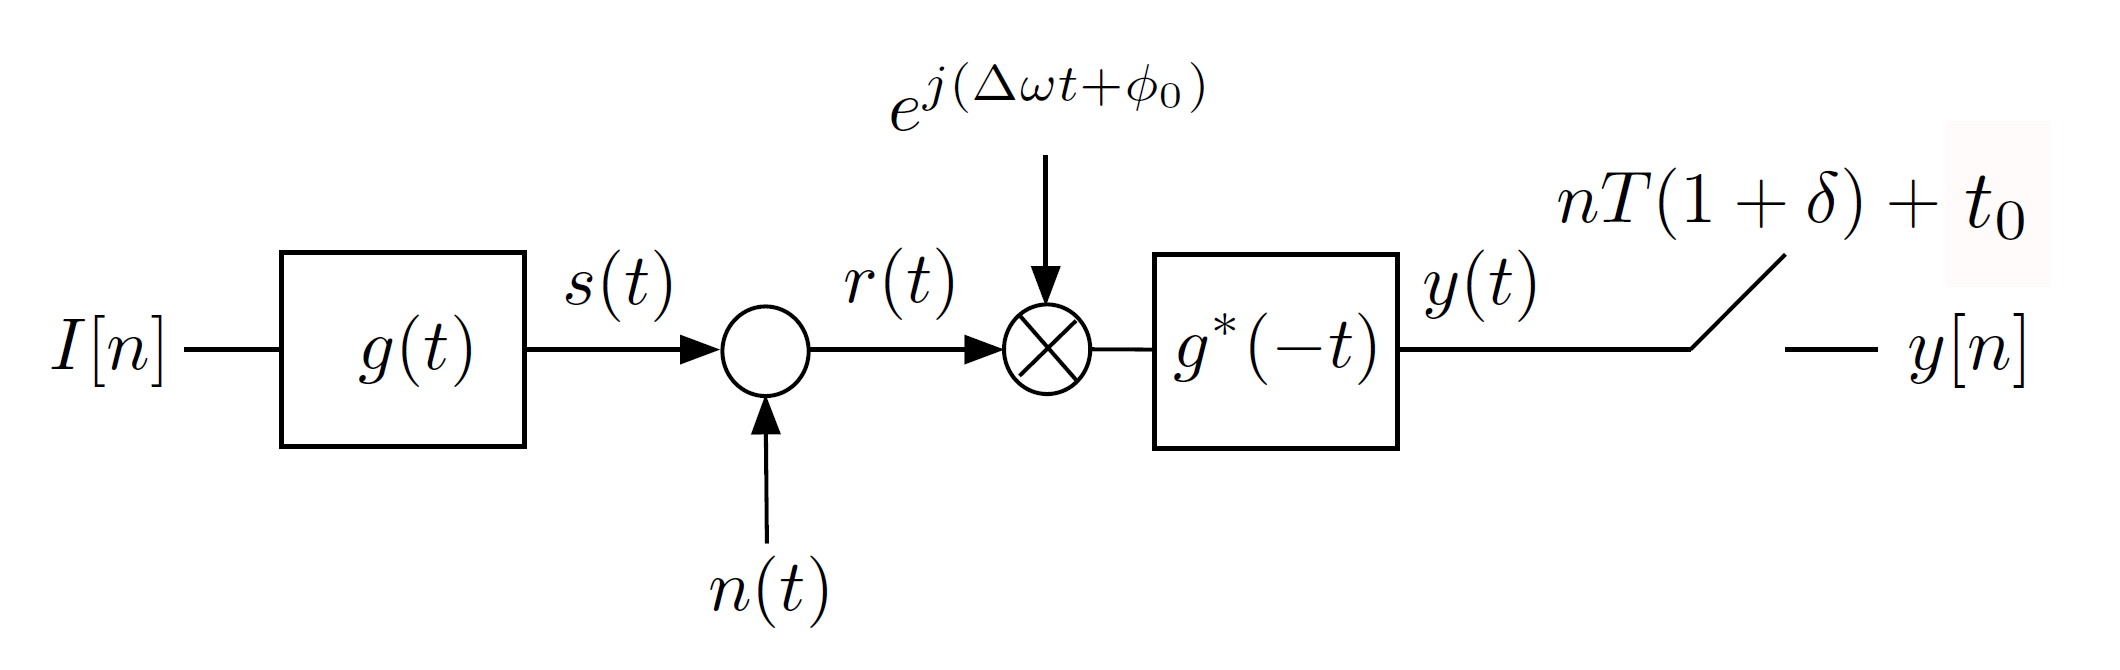
\includegraphics[width=0.8\linewidth]{Images/sync-errors-conceptual} % Ensure 'Images/sync-errors-conceptual' path is correct
	\caption{Synchronization mismatches at the receiver}
	\label{fig:sync-errors-conceptual}
\end{figure}

\newpage
\subsection{Impact of Synchronization Errors on Performance}
\textcolor{red}{[TODO: COMPLETE LATER THE CONSEQUENCES WITH LECTURE'S MATH]}\par

\subsubsection{Impact of Carrier Phase Offset ($\phi_0$)}
A static carrier phase offset, $\phi_0$, resulting from the phase difference between the incoming carrier and the receiver's local oscillator, causes a rotation of the entire received symbol constellation by an angle $\phi_0$ in the complex plane. Assuming perfect timing, no CFO, and no noise, a transmitted complex baseband symbol $I[n]$ becomes at the matched filter output:
\begin{equation}
	y[n] = I[n]e^{j\phi_0}
\end{equation}

\subsubsection{Impact of Carrier Frequency Offset ($\Delta f$)}
A carrier frequency offset $\Delta f$ means the received signal before matched filtering can be modeled as $r(t) = s(t) e^{j(2\pi \Delta f t}$, (assuming no phase offset and no noise). The impacts of CFO are:
\begin{enumerate}
	\item Phase Drift: After matched filtering and sampling at $t = nT_{symb}$, each symbol $I[n]$ experiences a progressively changing phase rotation: $y[n] = I[n] e^{j(2\pi \Delta f nT_{symb})}$. This causes the received constellation points to form a spiral pattern if uncorrected, as depicted in Figure \ref{fig:cfo-combined}.
	\item Inter-Symbol Interference (ISI): If the CFO is significant, the received signal's spectrum is shifted. Consequently, the receiver's filter $g^*(-t)$ is no longer perfectly matched to the incoming signal component $g(t)e^{j2\pi \Delta f t}$, leading to a loss in SNR and the introduction of ISI.
\end{enumerate}


\subsubsection{Impact of Sample Time Shift ($t_0$)} % Corrected from \subsection to \subsubsection
An incorrect sampling instant $t_0 \neq 0$ (relative to the optimal point) means the matched filter output is not sampled at maximum signal energy and zero ISI. If $h(t)$ is the overall Nyquist filter response, sampling at $nT_{symb} + t_0$ (assuming no noise) yields:
\begin{align}
	y[n] &= \sum_m I[m]h((n-m)T_{symb} + t_0) \\
	&= I[n]h(t_0) + \sum_{m \neq n} I[m]h((n-m)T_{symb} + t_0)
\end{align}
The first term, $I[n]h(t_0)$, represents the attenuated desired symbol (since $h(t_0) < h(0)$ for $t_0 \neq 0$). The second term is the ISI, as $h(kT_{symb} + t_0)$ is non-zero for $k \neq 0$ when $t_0 \neq 0$.

\begin{figure}[H]
	\centering
	\begin{subfigure}[b]{0.48\textwidth}
		\centering
		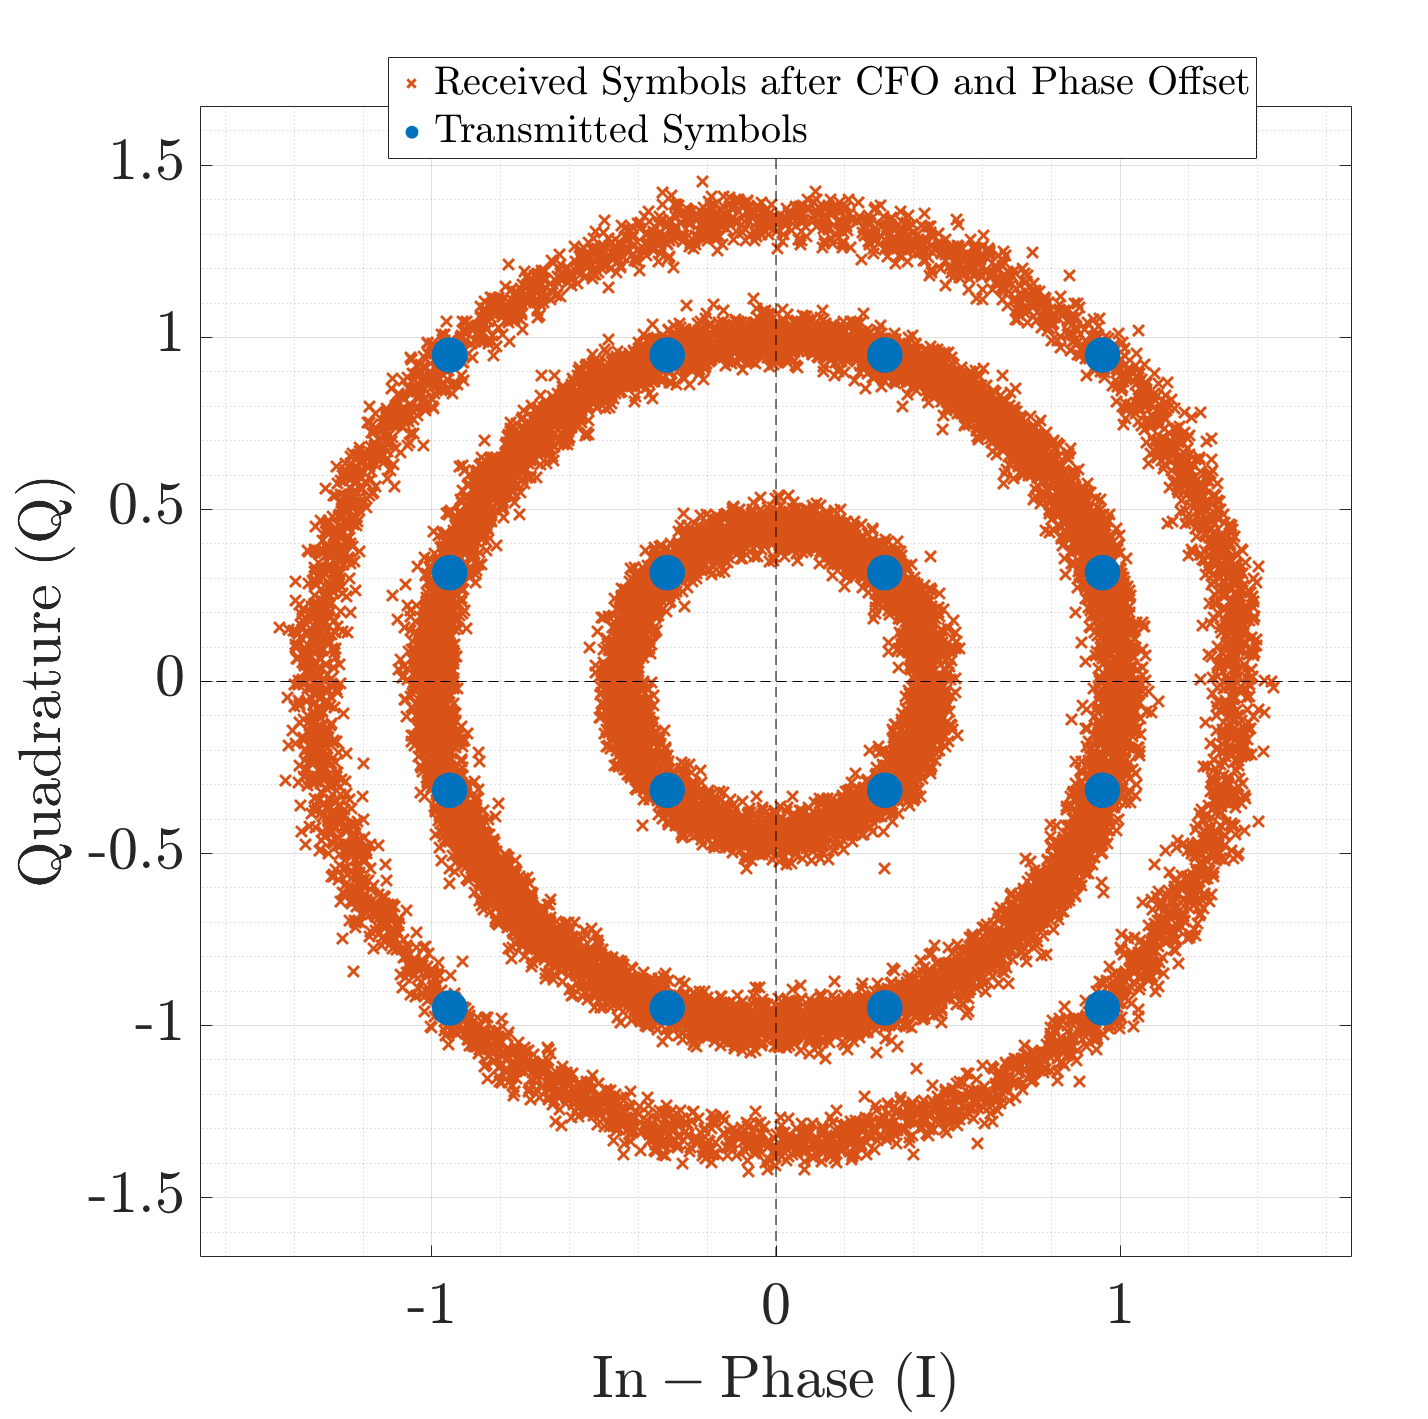
\includegraphics[width=\linewidth]{Images/cfo-po}
		\caption{16-QAM Constellation diagram after CFO and Phase Offset}
		\label{fig:cfo-po-sub}
	\end{subfigure}
	\hfill % or \hspace{\fill} or \quad
	\begin{subfigure}[b]{0.48\textwidth}
		\centering
		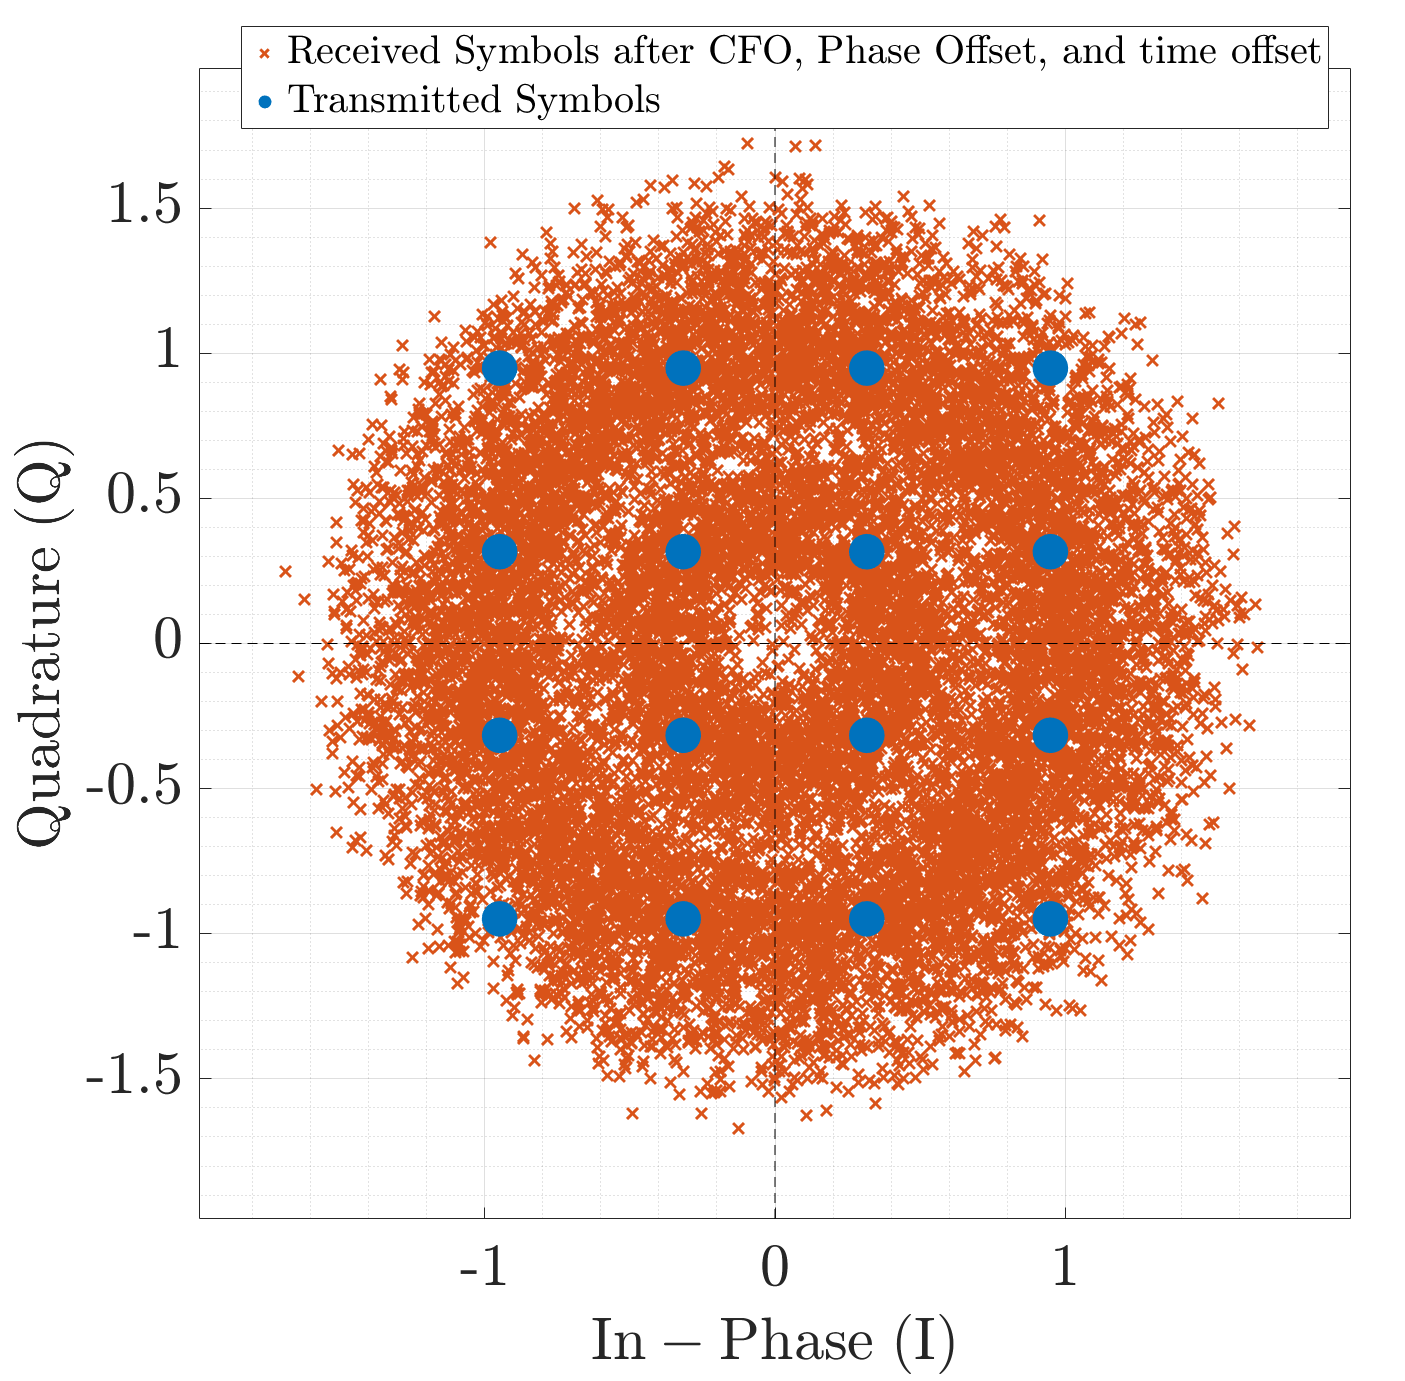
\includegraphics[width=\linewidth]{Images/cfo-po-to}
		\caption{16-QAM Constellation diagram after CFO, Phase Offset and time offset}
		\label{fig:cfo-po-to-sub}
	\end{subfigure}
	\caption{Constellation diagrams of symbols transmitted and received after adding AWGN noise such that $\frac{E_b}{N_0} = 20$ dB, and filtering.}
	\label{fig:cfo-combined}
\end{figure}


\subsection{Gardner Algorithm for Sampling Time Tracking}
\textcolor{red}{[CONTENT FROM DOCUMENT]}
\subsection{Frame and Frequency Acquisition using Differential Cross-Correlator}
\textcolor{red}{[CONTENT FROM DOCUMENT]}
\subsection{Phase Interpolation}
\textcolor{red}{[CONTENT FROM DOCUMENT]}